\section{HexGANFuzzer Framework}
In this section, we first acquire a large number of communication data from the ICS to be tested and then preprocess the data as the training data of the deep adversarial learning model established. Secondly, a generative model and a discriminant model are designed to generate the adversarial network, and a specific model is obtained by training and retraining the model with the acquired data. Finally, a series of performance metrics are put forward to evaluate our model.


\subsection{Preprocessing of ICP Message Frames}
In order to get diverse test cases, reach high code coverage and desirable fuzzing results, data preprocessing is a necessary part. There are two steps in preprocessing: \textbf{Message Frame Clustering} and \textbf{Data Conversion}.

\subsubsection{\textbf{Message Frame Clustering}}
After message frames collection, there are many different length message frames of the ICP. We adopted the Length Clustering method to preprocess the data frames. It is noted that most message frames with the same length share the same frame type. First, we gather the data frames which have the same length. In order not to get too many groups of data frames, groups whose quantity is less than a threshold (e.g. 5000) will be moved to the longer adjacent group, while group contains more data than the threshold are left unchanged. In such a way, there may be message frames with different lengths in one group. After clustering, the max length of message frames of every group will be the standard length and message frames whose length is less than max length will be added special token `u' at the end of them.

\subsubsection{\textbf{Data Conversion}}
The raw data frame of most protocols is hexadecimal, which can not be fed into the model directly. So after clustering, the hexadecimal data frames will be mapped into the digital vectors. The vocabulary we use is as followed:
\begin{equation}
\textit{\textbf{0 1 2 3 4 5 6 7 8 9 a b c d e f u}}
\end{equation}
The size of the vocabulary is 17, there are ten digits and seven hexadecimal characters according to the hexadecimal message frames and the supplement token `u'.
Based on the vocabulary, message frames $x \in R^{seq\_size \times 1}$ were converted into one hot vector $X \in R^{seq\_size \times 17}$(seq\_size is the max length of the current group), and one-hot vectors of real message frame will be the input of the critic.

\begin{figure}[htbp]   %  插入一栏图片
	\centering 
	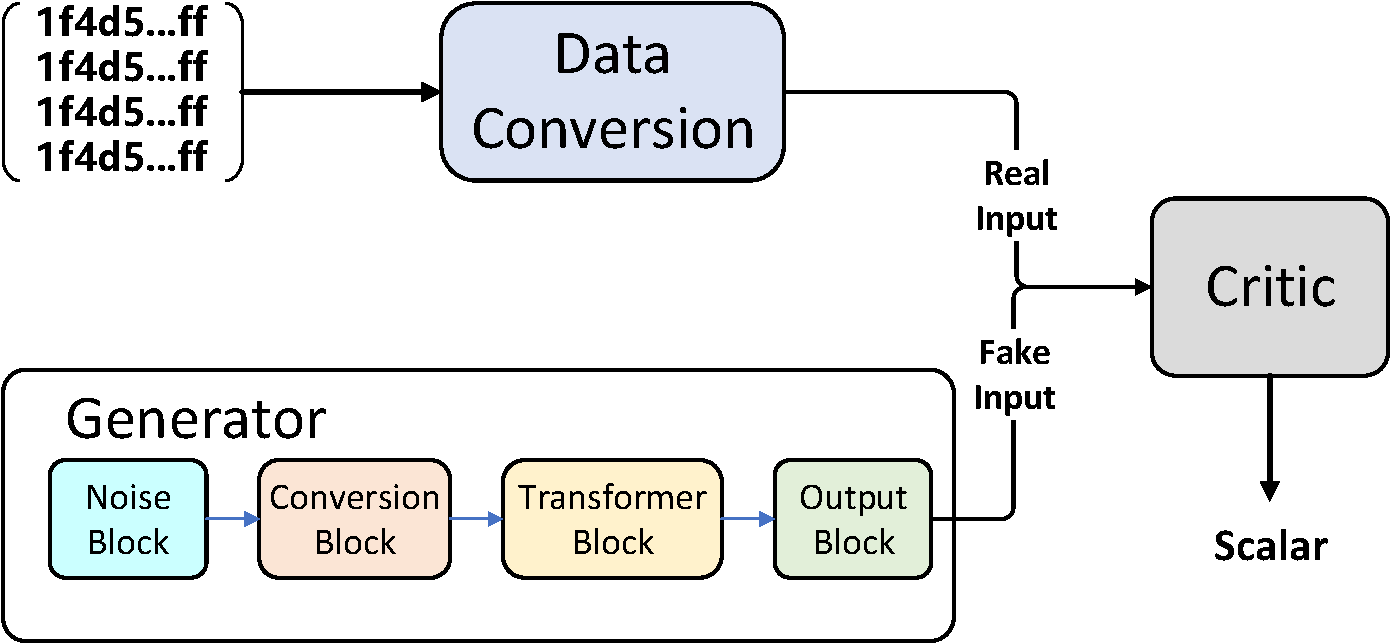
\includegraphics[width=3.5in]{FigHexGANFuzzer_model.pdf}
	\caption{The architecture of HexGANFuzzer}
	\label{FigHexGANFuzzer_model}
\end{figure}
\subsection{Model Design} 
\label{sec:model_design} 
In this part, we describe our test case generation model in detail. As Fig. \ref{FigHexGANFuzzer_model} shows, our model consists of a generator and a critic, which is the same as a WGAN model. The generator is born to generate the fake message frames and the critic will evaluate the Wasserstein distance. The Wasserstein distance is the minimum cost of transporting mass in converting the data distribution $q$ to the data distribution $p$. During the training, the Wasserstein distance between real message frame distribution and fake message frame distribution will be shortened and our model grasps the knowledge of the protocol grammar.

\begin{figure}[htbp]   %  插入一栏图片
	\centering 
	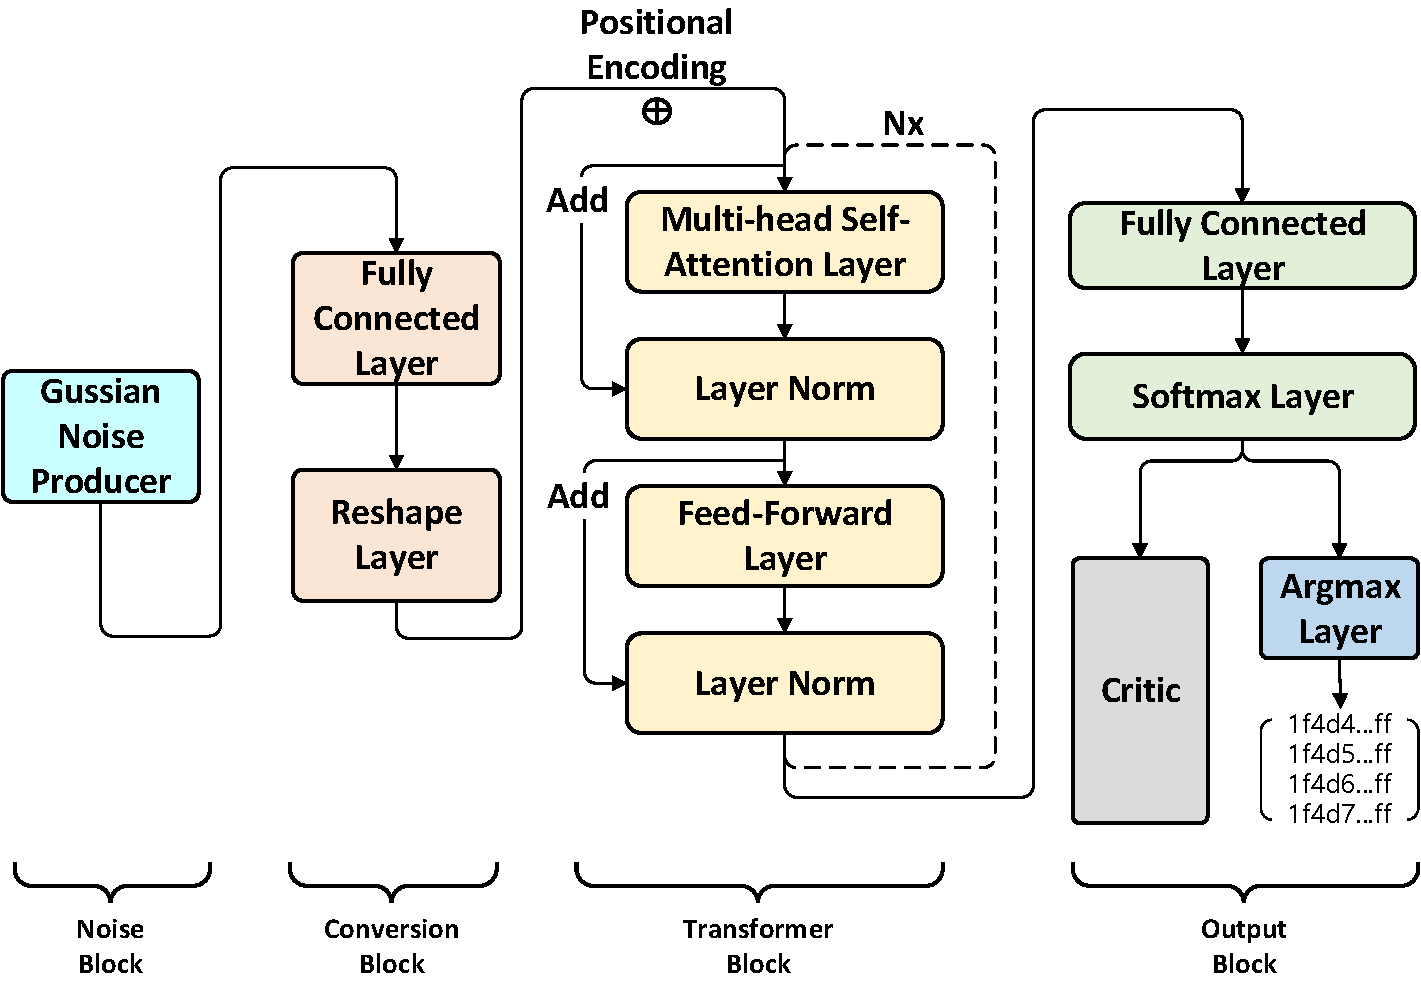
\includegraphics[width=3.5in]{FigHexGANFuzzer_Generator.pdf}
	\caption{Generator Network}
	\label{FigHexGANFuzzer_Generator}
\end{figure}
\subsubsection{\textbf{Generator}}

%总体描述,分为四个部分,四个部分里面分别是什么,简单介绍作用
The structure of the generator is as followed in Fig. \ref{FigHexGANFuzzer_Generator}. There are four parts, noise block, conversion block, transformer block, and output block. In order to generate different message frame data every time, the noise block will output some random noise data $z \in \mathbb{R}^{1 \times zd}$ where $zd$ is the initial dimension of the noise. And it is a common practice to set the noise data to Gaussian distributed noise. 

The conversion block contains a fully connected layer and a reshape layer. This block will convert the noise data $z$ into Noise Conversion Representation (NCR) $\tilde{z} \in \mathbb{R}^{ss \times dm}$ where $ss$ is the max sequence length of the current group and $dm$ is the number of feature dimension.

The transformer block contains a positional encoding layer and a sub-block (yellow boxes). The sub-block is the same as the encoder part of the Transformer \cite{vaswani2017attention}. It is formed by a multi-head self-attention layer and a feed-forward layer. Besides, there is a residual connection around each of the two layers, followed by layer normalization. And the input and output of the transformer block are the same, so this part can repeat as many times as we want.

The output block is a fully connected layer and a softmax layer. After the conversion block and the transformer block, the generator will not output the message frame data directly, instead, it outputs a probability vector $\tilde{x} \in \mathbb{R}^{ss \times vs}$. Where $vs$ is the size of vocabulary, which is $17$ in our situation. The probability vector is an intermediate result which is used to feed to the critic. To obtain the message frame which can be sent, the probability vector will be applied $argmax$ function and be translated into hexadecimal data according to the vocabulary mentioned before.

The sequence information is normally one-dimensional vector, but during the computation in the NLP model, the sequence information is represented by two-dimensional vectors including word embedding or one-hot vector for the sake of a better representation of the sequence. 
For example, the input words of \cite{vaswani2017attention} are converted into word embedding. In our model, the two-dimensional vector is NCR. 
The reason we use NCR is that the output of the noise block is a random noise vector, which is hard to get the corresponding word embedding. In the NLP tasks, discrete data is usually regarded as the result of continuous sampling from the categorical distribution. If we force to find the word embedding with some tricks, it may cause the whole procedure non-derivable, which will make the backpropagation algorithm unavailable. 
The solution of most GAN text generation model is using the one-hot vector to replace the word embedding in the model. In this paper, our solution is NCR. Define the fully connected layer as $f$, processed by fully connected layer, ReLU activation and reshape operation, noise data $z$ will become $\tilde{z} = Reshape(f(z))$ and $ \tilde{z} \in \mathbb{R}^{ss \times {dm}}$. And it is the input of the transformer block.
NCR looks like word embedding, but it is fake. NCR maps the one-dimension noise vector to high dimensional space information. Compared with the one-hot vector, NCR can cover more information of high dimension space.


The transformer block is a feature extractor. Compared with the commonly used feature extractor, Recurrent Neural Network (RNN), the transformer block is better in semantic feature extraction and long-range feature extraction. Moreover, the self-attention layer in the transformer block supports parallel training, which can accelerate the training process.
The loss function of the generator is 
\begin{equation}
L_{g} = - \mathop{\mathbb{E}}\limits_{\tilde{x}\sim\mathbb{P}_{g}}\left [ D(\tilde{x}) \right ] 
\end{equation}
where D is a 1-Lipschitz function, $\tilde{x} \in \mathbb{R}^{ss \times vs}$ is the output of the generator, $\mathbb{P}_g$ is the model distribution implicitly defined by $\tilde{x}=G(z)$, and $z$ is the noise data.

\begin{figure}[htbp]   %  插入一栏图片
	\centering 
	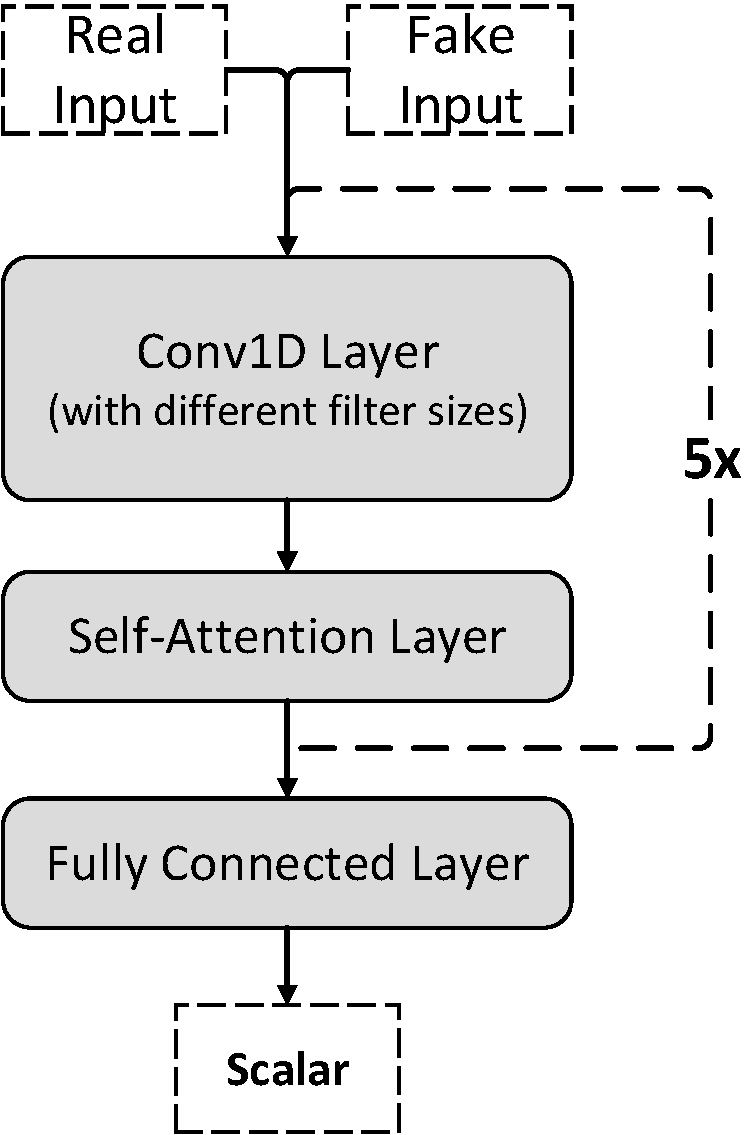
\includegraphics[width=1.5in]{FigHexGANFuzzer_Critic.pdf}
	\caption{Generator Network}
	\label{FigHexGANFuzzer_Critic}
\end{figure}
\subsubsection{\textbf{Critic}}
It looks like discriminator in normal GAN model, but it is not a classifier, we call it critic here, which is the same as WGAN \cite{arjovsky2017wasserstein}. The structure of the critic is as Fig. \ref{FigHexGANFuzzer_Critic} shows. The critic includes five conv1d layers, five self-attention layers, and one fully connected layer. For the critic, there are two types of inputs. One is the one-hot vector from the real message frames, and another is the output of the generator which represents the fake message frames. 
The second dimension of the output of the generator means the probability of each word in the vocabulary, and one-hot vector can also be understood as a special case of it, that is, the probability of one word is 1 and the probability of other words is 0. 

It is noted that the first conv1d layer changes the second dimension of inputs from the probability of word to the feature representation, which is the same as the dimension of NCR. And other conv1d layers keep the second dimension as $dm$. Every conv1d layer followed by a self-attention layer but the kernel size of conv1d is not the same. The kernel size of $i$th conv1d layer $ks_i = i$ where $i \in \{1,2,3,4,5\}$. 

Protocols have message headers, which specify the content of the message body in the message frame. More simply, the front part of the message frame affects the back part. It is hard to distinguish the boundary of two parts without the knowledge of the protocol grammar. If the model has learned which part is the message header, it can pay more attention to the message header part.
Due to different protocols have different lengths of the message header, the conv1d layer with different kernel size can capture the information better.
As for the content in the message header, several flags in the message header affect different parts of the content in the message body. self-attention layers can capture how flags in the message header affect the part of the message body.

The self-attention layer considers the attention weight of every position of the input and is good at learning long-range dependencies. With the boundary information leaned by conv1d layers, self-attention layers will pay more attention to the correlation between the content in the message header and body. After repeated self-attention and conv1d layers five times, the fully connected layer will output a scalar score. 
The loss of the critic is:
\begin{equation}
L_{c} = \mathop{\mathbb{E}}\limits_{\tilde{x}\sim\mathbb{P}_{g}}\left [ D(\tilde{x}) \right ] 
- \mathop{\mathbb{E}}\limits_{x\sim\mathbb{P}_{r}}\left [ D(x) \right ] 
+ \lambda\mathop{\mathbb{E}}\limits_{\hat{x}\sim\mathbb{P}_{\hat{x}}}\left [ ( \left \| \triangledown_{\hat{x}}D( \hat{x}) \right \|_{2} - 1 )^{2} \right ]
\end{equation}
where $\mathbb{P}_{\tilde{x}}$ define sampling uniformly along straight lines between pairs of points sampled from the real data distribution $\mathbb{P}_{r}$ and the generator distribution $\mathbb{P}_{g}$. 
In order to satisfy the 1-Lipschitz constraint, the solution of the WGAN-GP model was adopted. 
We use gradient penalty instead of the weight clipping to enforce the 1-Lipschitz constraint. 
It leads to a more stable training process and the model is easier to train.

\subsubsection{\textbf{Training strategy}}
Once the model design is completed, we begin to train our model. Under normal circumstances, the training of the GAN is adversarial, which means the generator and discriminator (critic) should be on the same level. If the imbalance is too serious, another one will learn nothing. And this is the reason why the GAN model is difficult to train and the training is unstable.
Due to the properties of the Wasserstein distance, we can train the critic better first and then narrow the Wasserstein distance between fake message frame distribution and real message frame distribution, which is the process of improving generator. In every epoch, we train generator once and then train the critic $c\_iters$ ($5$ in our model) times. Adam Optimizer was used both in the generator and the critic. In order to judge the convergence of the model, the following equation, which is the approximate value of the Wasserstein distance, is an indicator. If the value of the equation trends to be stable, we consider the model is convergent.
\begin{equation}
W\_distance = 
\mathop{\mathbb{E}}\limits_{x\sim\mathbb{P}_{r}}\left [ D(x) \right ] 
- \mathop{\mathbb{E}}\limits_{\tilde{x}\sim\mathbb{P}_{g}}\left [ D(\tilde{x}) \right ] 
\end{equation}
Though the model wants to generate the fake message frames that share high similarity to the real message frames, the ulmate goal is to achieve effective fuzzing results and identify as many bugs as possible. In order to obtain the desired results, there should be some differences between the real data and the fake data. So we not only save the final version of the model, which is convergent, but also the intermediate generator model. The model was saved every 10 training epoch deliberately. In such a training strategy, the goal of the high code coverage and deeper testing depth can be achieved.


\subsection{Performance Metrics}
Some quantitative criteria \cite{heusel2017gans} \cite{karras2017progressive} \cite{lucic2018gans} have emerged recently for evaluating the performance of GAN on image generation. However, there is no corresponding evaluation metrics in fuzzing based on deep adversarial learning, and the lack of these indicators includes two aspects: the evaluation of the performance of the machine learning model \cite{karras2017progressive} \cite{lucic2018gans} in the field of fuzzing based on deep learning \cite{shmelkov2018good} and the evaluation of the vulnerability detection capability. Therefore, in accordance with our research purpose and specific situation, the following evaluation metrics are proposed in this study.

%represents the percentage of correctly generating characters about function codes in generated test case sequences versus function codes in real test case packages
\subsubsection{\textbf{F-measure}}
In order to further demonstrate the performance of our model in this paper, we compare the performance of different models on test data generation of ICPs with several indexs such as \textit{Sensitivity}, \textit{Specificity}, \textit{Accuracy} and \textit{F-measure}.  Among them, Sensitivity represents the percentage of function codes for correctly generated test case packages versus function codes for real test case packages, Specificity means to the percentage of non-essential hexadecimal characters for correctly generated test case packages versus non-essential hexadecimal characters for real test case packages, and Accuracy is the percentage of the entire test case that correctly generates the format and message content of the test case package. The specific formula is as follows:
\begin{equation}
Accuracy = \frac{{TP + TN}}{{TP + FN + TN + FP}}
\end{equation}
\begin{equation}
Sensitivity = \frac{{TP}}{{TP + FN}}
\end{equation}
\begin{equation}
Specificity = \frac{{TN}}{{TN + FP}}
\end{equation}
\begin{equation}
Precision = \frac{{TP}}{{TP + FP}}
\end{equation}
\begin{equation}
Recall = \frac{{TP}}{{TP + FN}}
\end{equation}
\begin{equation}
\begin{array}{l}
F - measure =\displaystyle{2 \times Precision \times}  \\
\\{\kern 1pt} {\kern 1pt} {\kern 1pt} {\kern 1pt} {\kern 1pt} {\kern 1pt} {\kern 1pt} {\kern 1pt} {\kern 1pt} {\kern 1pt} {\kern 1pt} {\kern 1pt} {\kern 1pt} {\kern 1pt} {\kern 1pt} {\kern 1pt} {\kern 1pt} {\kern 1pt} {\kern 1pt} {\kern 1pt} {\kern 1pt} {\kern 1pt} {\kern 1pt} {\kern 1pt} {\kern 1pt} {\kern 1pt} {\kern 1pt} {\kern 1pt} {\kern 1pt} {\kern 1pt} {\kern 1pt} {\kern 1pt} {\kern 1pt} {\kern 1pt} {\kern 1pt} {\kern 1pt} {\kern 1pt} {\kern 1pt} {\kern 1pt} {\kern 1pt} {\kern 1pt} {\kern 1pt} {\kern 1pt} {\kern 1pt} {\kern 1pt} {\kern 1pt} {\kern 1pt} {\kern 1pt} {\kern 1pt} {\kern 1pt} {\kern 1pt} {\kern 1pt} {\kern 1pt} {\kern 1pt} {\kern 1pt} {\kern 1pt} {\kern 1pt} {\kern 1pt} {\kern 1pt} \displaystyle\frac{{Recall}}{{Precision + Recall}}
\end{array}
\end{equation}
wherein, TP is the number of correctly generated hexadecimal characters that constitute the function codes of ICPs' packages, TN is the number of correctly generated other non-essential hexadecimal characters including message content of ICPs' packages, FP is the number of hexadecimal characters  generated by error that constitute the function codes of ICPs' packages, and FN is the number of generated by error other non-essential hexadecimal characters including message content of ICPs' packages.

\subsubsection{\textbf{Effectiveness of Vulnerability Detection (EVD)}}
EVD refers to the ability to trigger anomalies on basis of the test target accepting the test data. The effectiveness of fuzzing depends predominantly on the testing depth and high code coverage. Therefore, we propose the effectiveness evaluation metric EVD for fuzzing models from the above two aspects.
%  The effectiveness evaluation of the fuzzing methods can be divided into two aspects: testing depth and code coverage.

When the generated data can be accepted by the test target, it indicates that the generated data is similar to real data in terms of the format, embodying that the model has the ability to learn the format of data frames from the real world. This phenomenon also reflects a certain depth of testing. But our ultimate goal is to trigger as many anomalies as possible to the ICS to find vulnerabilities, so two sub-metrics are taken into account when we finally calculate the testing depth for EVD: \textit{Acceptance Rate of Test Cases (ARTC)} and \textit{Ability of Vulnerability Detected (AVD)}:

\quad \textit{\textbf{a. ARTC.}} ARTC refers to the acceptance rate at which the generated test data is received by the test target when it is sent to the test target. The specific formula is as follows:
\begin{equation}
ARTC = \frac{{N_{accepted}}}{{N_{all}}} \times 100\%  
\end{equation}
where ${N_{accepted}}$ is the total number of test cases accepted and ${N_{all}}$ is the total number of test cases sent.

\quad \textit{\textbf{b. AVD.}} AVD refers to the ability of triggering anomalies for the test target when the generated test data is sent to the test target. We define AVD as follows:
\begin{equation}
AVD = \frac{{N_{anomalies}}}{{N_{all}}} \times 100\%  
\end{equation}
where ${N_{anomalies}}$ is the total number of test cases which trigger anomalies and ${N_{all}}$ is the total number of test cases sent.

\textit{\textbf{Diversity of Generated Cases (DGC)}} is a sub-metric proposed as the extent of code coverage for fuzzing in EVD. It refers to the ability to maintain the diversity of the generated data. The diversity-based approach is a useful test case selection criterion for code coverage \cite{hemmati2013achieving} \cite{mondal2015exploring}. Furthermore, more diverse generated test data frames are likely to cause more exceptions. And this indicator focuses on the number of message types in the generated data, see the following formula: 
\begin{equation}
DGC = \frac{{N_{gen\_categories}}}{{N_{all\_categories}}} \times 100\% 
\end{equation}
where $N_{gen\_categories}$ is the total number of message categories in the generated data frames, and $N_{all\_categories}$ is the total number of message categories in the training dataset.

In order to balance the different weights of sub-metrics on model effectiveness, dimensionless quantity method is applied to eliminate the influence of different scales between sub-metrics so that each sub-metric can be converted into a value that can be directly added or subtracted. We normalize aforementioned sub-metrics and add them up to get the comprehensive scores for EVD:
\begin{equation}
\begin{array}{l}
EVD=(\displaystyle\frac{{ART{C_i} - ART{C_{\min }}}}{{ART{C_{\max }} - ART{C_{\min }}}} + \frac{{VD{E_i} - VD{E_{\min }}}}{{VD{E_{\max }} - VD{{E}_{\min }}}}\\
\\{\kern 1pt} {\kern 1pt} {\kern 1pt} {\kern 1pt} {\kern 1pt} {\kern 1pt} {\kern 1pt} {\kern 1pt} {\kern 1pt} {\kern 1pt} {\kern 1pt} {\kern 1pt} {\kern 1pt} {\kern 1pt} {\kern 1pt} {\kern 1pt} {\kern 1pt} {\kern 1pt} {\kern 1pt} {\kern 1pt} {\kern 1pt} {\kern 1pt} {\kern 1pt} {\kern 1pt} {\kern 1pt} {\kern 1pt} {\kern 1pt} {\kern 1pt} {\kern 1pt} {\kern 1pt} {\kern 1pt} {\kern 1pt} {\kern 1pt} {\kern 1pt} {\kern 1pt} {\kern 1pt} {\kern 1pt} {\kern 1pt} {\kern 1pt} {\kern 1pt} {\kern 1pt} {\kern 1pt} {\kern 1pt} {\kern 1pt} {\kern 1pt} {\kern 1pt} {\kern 1pt} {\kern 1pt} {\kern 1pt} {\kern 1pt} {\kern 1pt} {\kern 1pt} {\kern 1pt} {\kern 1pt} {\kern 1pt} {\kern 1pt} {\kern 1pt} {\kern 1pt} {\kern 1pt} {\kern 1pt} {\kern 1pt} {\kern 1pt} {\kern 1pt} {\kern 1pt} {\kern 1pt} {\kern 1pt} {\kern 1pt} {\kern 1pt} {\kern 1pt} {\kern 1pt} {\kern 1pt} {\kern 1pt} {\kern 1pt} {\kern 1pt} {\kern 1pt} {\kern 1pt} {\kern 1pt} {\kern 1pt} {\kern 1pt} {\kern 1pt} {\kern 1pt} {\kern 1pt} {\kern 1pt} {\kern 1pt} {\kern 1pt} {\kern 1pt} {\kern 1pt}  {\kern 1pt} {\kern 1pt} {\kern 1pt}  
+ {\kern 1pt} \displaystyle\frac{{DG{C_i} - DG{C_{\min }}}}{{DG{C_{\max }} - DG{C_{\min }}}}) \times \displaystyle\frac{{100}}{3}{\kern 1pt}
\end{array}
\end{equation}
setting the values of different effectiveness sub-metrics of a model as \{${{sm}_1}$, ${{sm}_2}$, ... , ${{sm}_n}$\}, then values of ARTC, AVD and DGC of the ith model are: ${ARTC_i}$, ${AVD_i}$ and ${DGC_i}$. ${{sm}_{max}}$ and ${{sm}_{min}}$ are respectively the maximum and minimum values of the corresponding sub-metric.

\subsubsection{\textbf{Efficiency of Vulnerability Detection (EFVD)}}
EFVD is an important metric of model Efficiency. On one hand, it refers to the \textit{Training Time (TT)} required to train a model. On the other hand, it indicates the \textit{Time of Anomalies Triggered (TAT)} after sending a fixed number of test cases. 

\quad \textit{\textbf{a. TT.}} Short TT correspondingly improves the efficiency of testing.

% for each fuzzy test 
\quad \textit{\textbf{b. TAT.}} TAT refers to the time interval from the first request time (${t_1}$) to the time when the third anomaly (such as error code 3, no response from the server, etc.) is triggered (${t_{{3_{{\rm{th\_anomaly}}}}}}$) . The following formula is for TAT in this paper:
\begin{equation}
TAT={t_{{3_{{\rm{th\_anomaly}}}}}} - {t_1}  
\end{equation}
It should be noted that the number of anomalies found is also related to the test target. Weak target will highlight the method effectiveness. However, because our ultimate goal is not to find the differences between the various test target, we only focus on the efficiency of the method in this study. The specific formula is as follows:

\begin{equation}
\begin{array}{l}
EFVD=(\displaystyle\frac{{T{T_i} - T{T_{\min }}}}{{T{T_{\max }} - T{T_{\min }}}} + \frac{{TA{T_i} - TA{T_{\min }}}}{{TA{T_{\max }} - TA{T_{\min }}}})\\
\\{\kern 1pt} {\kern 1pt} {\kern 1pt} {\kern 1pt} {\kern 1pt} {\kern 1pt} {\kern 1pt} {\kern 1pt} {\kern 1pt} {\kern 1pt} {\kern 1pt} {\kern 1pt} {\kern 1pt} {\kern 1pt} {\kern 1pt} {\kern 1pt} {\kern 1pt} {\kern 1pt} {\kern 1pt} {\kern 1pt} {\kern 1pt} {\kern 1pt} {\kern 1pt} {\kern 1pt} {\kern 1pt} {\kern 1pt} {\kern 1pt} {\kern 1pt} {\kern 1pt} {\kern 1pt} {\kern 1pt} {\kern 1pt} {\kern 1pt} {\kern 1pt} {\kern 1pt} {\kern 1pt} {\kern 1pt} {\kern 1pt} {\kern 1pt} {\kern 1pt} {\kern 1pt} {\kern 1pt} {\kern 1pt} {\kern 1pt} {\kern 1pt} {\kern 1pt} {\kern 1pt} {\kern 1pt} {\kern 1pt} {\kern 1pt} {\kern 1pt} {\kern 1pt} {\kern 1pt} {\kern 1pt} {\kern 1pt} {\kern 1pt} {\kern 1pt} {\kern 1pt} {\kern 1pt} {\kern 1pt} {\kern 1pt} {\kern 1pt} {\kern 1pt} {\kern 1pt} {\kern 1pt} {\kern 1pt} {\kern 1pt} {\kern 1pt} {\kern 1pt} {\kern 1pt} {\kern 1pt} {\kern 1pt} {\kern 1pt} {\kern 1pt} {\kern 1pt} {\kern 1pt} {\kern 1pt} {\kern 1pt} {\kern 1pt} {\kern 1pt} {\kern 1pt} {\kern 1pt} {\kern 1pt} {\kern 1pt} {\kern 1pt} {\kern 1pt} {\kern 1pt}  {\kern 1pt} {\kern 1pt} {\kern 1pt}  
\times \displaystyle\frac{{100}}{2}{\kern 1pt}
\end{array}
\end{equation}
similar to aforementioned effectiveness sub-metrics, the values of TT and TAT of the ith model are: ${TT_i}$ and ${TAT_i}$. ${{TT}_{max}}$ and ${{TAT}_{min}}$ are respectively the maximum and minimum values of the corresponding sub-metric.

